\begin{frame}[fragile]{It's Easy to Hierarchically Build Models with Universes}

  \begin{scriptsize}
    \begin{lstlisting}[language=XML,gobble=4]
      <?xml version="1.0" encoding="UTF-8"?>
      <geometry>

        <!-- Fuel Rod Pincell Universe -->
        <surface id="1"  type="z-cylinder" coeffs="0.0 0.0 0.39218"/>     <!-- fuel OR   -->
        <surface id="2"  type="z-cylinder" coeffs="0.0 0.0 0.40005"/>     <!-- gap OR    -->
        <surface id="3"  type="z-cylinder" coeffs="0.0 0.0 0.45720"/>     <!-- clad OR   -->
        <cell id="21" universe="2" material="2" surfaces="  -1"/>         <!-- fuel  -->
        <cell id="22" universe="2" material="3" surfaces="1 -2"/>         <!-- clad  -->
        <cell id="23" universe="2" material="1" surfaces="   2"/>         <!-- water -->

      </geometry>
    \end{lstlisting}
  \end{scriptsize}


  \begin{itemize}
    \item Instead of using a \textit{material}, cells can be \textit{filled} with a universe
    \item By default universes share the same global coordinate system
    \begin{itemize}
      \item Can be translated and rotated - e.g. in lattices
    \end{itemize}
    \item Universes \textbf{must} be defined for \textbf{all} space
    \begin{itemize}
      \item Or you may encounter particle tracking errors!
    \end{itemize}
    \item Provides the easiest way to define multiple pincells, lattices, and 
    more complicated structures
  \end{itemize}


\end{frame}

%-------------------------------------------------------------------------------

\begin{frame}[fragile]{Cell Filling Example}


  \begin{scriptsize}
    \begin{lstlisting}[language=XML,gobble=4]
      <?xml version="1.0" encoding="UTF-8"?>
      <geometry>

        <!-- Fuel Rod Pincell Universe -->
        <surface id="1"  type="z-cylinder" coeffs="0.0 0.0 0.39218"/>     <!-- fuel OR   -->
        <surface id="2"  type="z-cylinder" coeffs="0.0 0.0 0.40005"/>     <!-- gap OR    -->
        <surface id="3"  type="z-cylinder" coeffs="0.0 0.0 0.45720"/>     <!-- clad OR   -->
        <cell id="21" universe="2" material="2" surfaces="  -1"/>         <!-- fuel  -->
        <cell id="22" universe="2" material="3" surfaces="1 -2"/>         <!-- clad  -->
        <cell id="23" universe="2" material="1" surfaces="   2"/>         <!-- water -->

        <!-- Main Universe -->
        <surface id="4"  type="x-plane" coeffs="-0.62992" boundary="reflective"/>
        <surface id="5"  type="x-plane" coeffs=" 0.62992" boundary="reflective"/>
        <surface id="6"  type="y-plane" coeffs="-0.62992" boundary="reflective"/>
        <surface id="7"  type="y-plane" coeffs=" 0.62992" boundary="reflective"/>
        <surface id="8"  type="z-plane" coeffs="-5.00000" boundary="reflective"/>
        <surface id="9"  type="z-plane" coeffs=" 5.00000" boundary="reflective"/>
        <cell id="1" universe="0" fill="2" surfaces="4 -5 6 -7 8 -9" />


      </geometry>
    \end{lstlisting}
  \end{scriptsize}

  \centering
  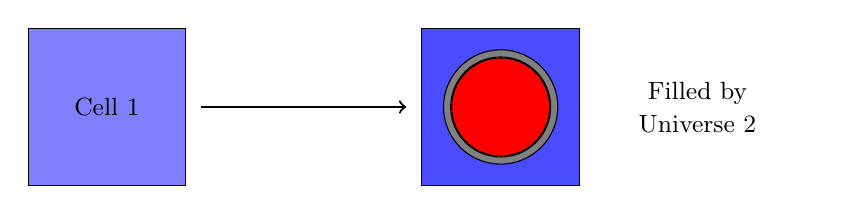
\begin{tikzpicture}
    \fill[white] (-1,-1) rectangle (9,1);
    \draw[fill=blue!50!white] (-1,-1) rectangle (1,1);
    \node at (0,0) {\small Cell 1};
    \draw[->,thick] (1.2,0) -- (3.8,0);
    \draw[fill=blue!70!white] (4,-1) rectangle (6,1);
    \draw[fill=gray] (5,0) circle (0.7258);
    \draw[fill=yellow] (5,0) circle (0.63508);
    \draw[fill=red] (5,0) circle (0.62250);
    \node[align=center] at (7.5,0) {\small Filled by \\ \small Universe 2};
  \end{tikzpicture}

\end{frame}

%-------------------------------------------------------------------------------

\begin{frame}[fragile]{Cell Filling Example}


  \begin{scriptsize}
    \begin{lstlisting}[language=XML,gobble=4]
      <?xml version="1.0" encoding="UTF-8"?>
      <geometry>

        <!-- Fuel Rod Pincell Universe -->
        <surface id="1"  type="z-cylinder" coeffs="0.0 0.0 0.39218"/>     <!-- fuel OR   -->
        <surface id="2"  type="z-cylinder" coeffs="0.0 0.0 0.40005"/>     <!-- gap OR    -->
        <surface id="3"  type="z-cylinder" coeffs="0.0 0.0 0.45720"/>     <!-- clad OR   -->
        <cell id="21" universe="2" material="2" surfaces="  -1"/>         <!-- fuel  -->
        <cell id="22" universe="2" material="3" surfaces="1 -2"/>         <!-- clad  -->
        <cell id="23" universe="2" material="1" surfaces="   2"/>         <!-- water -->

        <!-- Main Universe -->
        <surface id="4"  type="x-plane" coeffs="-0.0"     boundary="reflective"/>
        <surface id="5"  type="x-plane" coeffs=" 0.62992" boundary="reflective"/>
        <surface id="6"  type="y-plane" coeffs="-0.62992" boundary="reflective"/>
        <surface id="7"  type="y-plane" coeffs=" 0.62992" boundary="reflective"/>
        <surface id="8"  type="z-plane" coeffs="-5.00000" boundary="reflective"/>
        <surface id="9"  type="z-plane" coeffs=" 5.00000" boundary="reflective"/>
        <cell id="1" universe="0" fill="2" surfaces="4 -5 6 -7 8 -9" />


      </geometry>
    \end{lstlisting}
  \end{scriptsize}

  \centering
  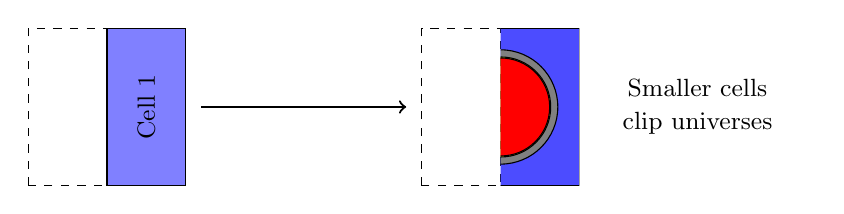
\begin{tikzpicture}
    \fill[white] (-1,-1) rectangle (9,1);
    \draw[fill=white, dashed] (-1,-1) rectangle (0,1);
    \draw[fill=blue!50!white] (0,-1) rectangle (1,1);
    \node[rotate=90] at (0.5,0) {\small Cell 1};
    \draw[->,thick] (1.2,0) -- (3.8,0);
    \draw[fill=white, dashed] (4,-1) rectangle (5,1);
    \begin{scope}
      \clip (5,-1) rectangle (6,1);
      \draw[fill=blue!70!white] (4,-1) rectangle (6,1);
      \draw[fill=gray] (5,0) circle (0.7258);
      \draw[fill=yellow] (5,0) circle (0.63508);
      \draw[fill=red] (5,0) circle (0.62250);
    \end{scope}
    \node[align=center] at (7.5,0) {\small Smaller cells \\ \small clip universes};
  \end{tikzpicture}

\end{frame}


%-------------------------------------------------------------------------------

\begin{frame}[fragile]{Cell Filling Example}

  \begin{scriptsize}
    \begin{lstlisting}[language=XML,gobble=4]
      <?xml version="1.0" encoding="UTF-8"?>
      <geometry>

        <!-- Fuel Rod Pincell Universe -->
        <surface id="1"  type="z-cylinder" coeffs="0.0 0.0 0.39218"/>     <!-- fuel OR   -->
        <surface id="2"  type="z-cylinder" coeffs="0.0 0.0 0.40005"/>     <!-- gap OR    -->
        <surface id="3"  type="z-cylinder" coeffs="0.0 0.0 0.45720"/>     <!-- clad OR   -->
        <cell id="21" universe="2" material="2" surfaces="  -1"/>         <!-- fuel  -->
        <cell id="22" universe="2" material="3" surfaces="1 -2"/>         <!-- clad  -->
        <cell id="23" universe="2" material="1" surfaces="   2"/>         <!-- water -->

        <!-- Main Universe -->
        <surface id="4"  type="x-plane" coeffs="-0.0"     boundary="reflective"/>
        <surface id="5"  type="x-plane" coeffs=" 0.62992" boundary="reflective"/>
        <surface id="6"  type="y-plane" coeffs="-0.62992" boundary="reflective"/>
        <surface id="7"  type="y-plane" coeffs=" 0.62992" boundary="reflective"/>
        <surface id="8"  type="z-plane" coeffs="-5.00000" boundary="reflective"/>
        <surface id="9"  type="z-plane" coeffs=" 5.00000" boundary="reflective"/>
        <cell id="1" universe="0" fill="2" surfaces="4 -5 6 -7 8 -9"
                                           translation="0.31496 0.0 0.0" />

      </geometry>
    \end{lstlisting}
  \end{scriptsize}

  \centering
  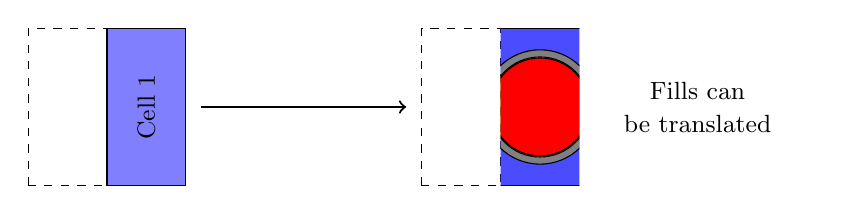
\begin{tikzpicture}
    \fill[white] (-1,-1) rectangle (9,1);
    \draw[fill=white, dashed] (-1,-1) rectangle (0,1);
    \draw[fill=blue!50!white] (0,-1) rectangle (1,1);
    \node[rotate=90] at (0.5,0) {\small Cell 1};
    \draw[->,thick] (1.2,0) -- (3.8,0);
    \draw[fill=white, dashed] (4,-1) rectangle (5,1);
    \begin{scope}
      \clip (5,-1) rectangle (6,1);
      \begin{scope}[shift={(0.5,0)}]
        \draw[fill=blue!70!white] (4,-1) rectangle (6,1);
        \draw[fill=gray] (5,0) circle (0.7258);
        \draw[fill=yellow] (5,0) circle (0.63508);
        \draw[fill=red] (5,0) circle (0.62250);
      \end{scope}
    \end{scope}
    \node[align=center] at (7.5,0) {\small Fills can \\ \small be translated};
  \end{tikzpicture}

\end{frame}

%-------------------------------------------------------------------------------

\begin{frame}[fragile]{Cell Filling Example}


  \begin{scriptsize}
    \begin{lstlisting}[language=XML,gobble=4]
      <?xml version="1.0" encoding="UTF-8"?>
      <geometry>

        <!-- Fuel Rod Pincell Universe -->
        <surface id="1"  type="z-cylinder" coeffs="0.0 0.0 0.39218"/>     <!-- fuel OR   -->
        <surface id="2"  type="z-cylinder" coeffs="0.0 0.0 0.40005"/>     <!-- gap OR    -->
        <surface id="3"  type="z-cylinder" coeffs="0.0 0.0 0.45720"/>     <!-- clad OR   -->
        <cell id="21" universe="2" material="2" surfaces="  -1"/>         <!-- fuel  -->
        <cell id="22" universe="2" material="3" surfaces="1 -2"/>         <!-- clad  -->
        <cell id="23" universe="2" material="1" surfaces="   2"/>         <!-- water -->

        <!-- Main Universe -->
        <surface id="4"  type="x-plane" coeffs="-0.0"     boundary="reflective"/>
        <surface id="5"  type="x-plane" coeffs=" 0.62992" boundary="reflective"/>
        <surface id="6"  type="y-plane" coeffs="-0.62992" boundary="reflective"/>
        <surface id="7"  type="y-plane" coeffs=" 0.62992" boundary="reflective"/>
        <surface id="8"  type="z-plane" coeffs="-5.00000" boundary="reflective"/>
        <surface id="9"  type="z-plane" coeffs=" 5.00000" boundary="reflective"/>
        <cell id="1" universe="0" fill="2" surfaces="4 -5 6 -7 8 -9"
                                           translation="0.31496 0.0 0.0"
                                           rotation="90.0 0.0 0.0" />
      </geometry>
    \end{lstlisting}
  \end{scriptsize}

  \centering
  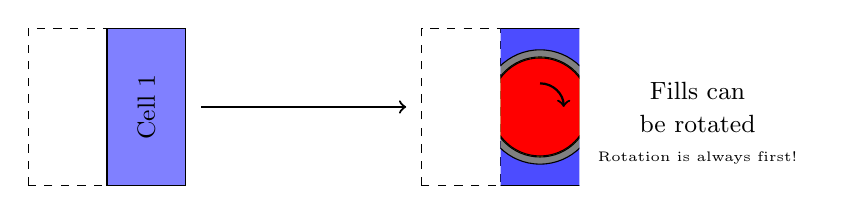
\begin{tikzpicture}
    \fill[white] (-1,-1) rectangle (9,1);
    \draw[fill=white, dashed] (-1,-1) rectangle (0,1);
    \draw[fill=blue!50!white] (0,-1) rectangle (1,1);
    \node[rotate=90] at (0.5,0) {\small Cell 1};
    \draw[->,thick] (1.2,0) -- (3.8,0);
    \draw[fill=white, dashed] (4,-1) rectangle (5,1);
    \begin{scope}
      \clip (5,-1) rectangle (6,1);
      \begin{scope}[shift={(0.5,0)}]
        \draw[fill=blue!70!white] (4,-1) rectangle (6,1);
        \draw[fill=gray] (5,0) circle (0.7258);
        \draw[fill=yellow] (5,0) circle (0.63508);
        \draw[fill=red] (5,0) circle (0.62250);
        \draw[->,thick] (5,0.3) arc[radius=0.3, start angle=90, end angle=0];
      \end{scope}
    \end{scope}m
    \node[align=center] (la) at (7.5,0) {\small Fills can \\ \small be rotated};
    \node[align=center,anchor=north] at (la.south) {\tiny Rotation is always first!};
  \end{tikzpicture}

\end{frame}
